\chapter{Proposed Methods} % Main chapter title

\label{Chapter4} % Change X to a consecutive number; for referencing this chapter elsewhere, use \ref{ChapterX}

\begin{figure}
  \centering
  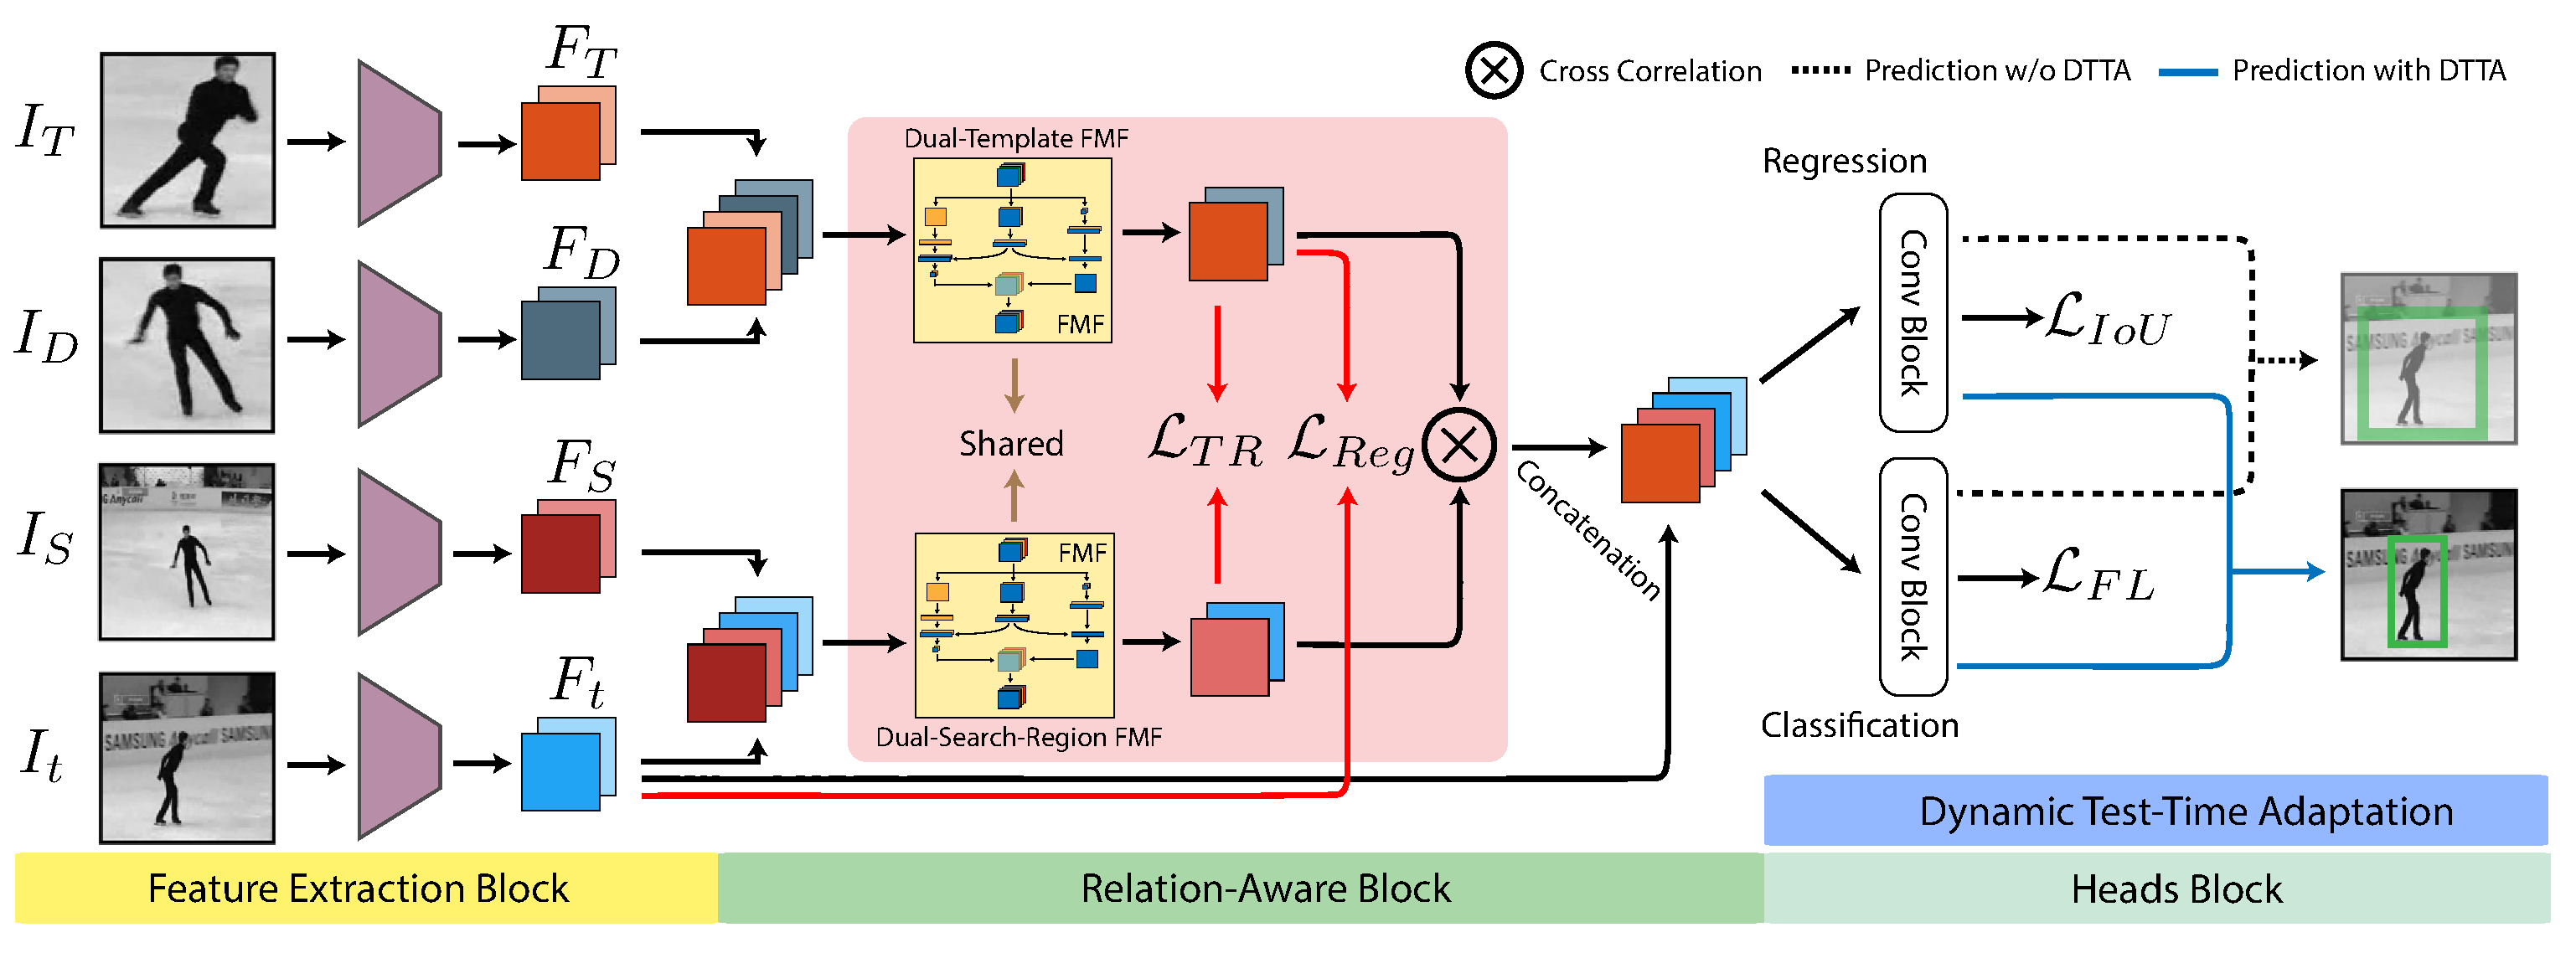
\includegraphics[width=1.0\textwidth]{figures/main_figure.pdf}
   \caption{\textbf{Overall Architecture.} The Feature Extraction Block uses a readily available backbone to process the frames. The Relation-Aware Block exploits representational relations among the dual-template and dual-search-region through our losses, $\mathcal{L}_{TR}$ and $\mathcal{L}_{Reg}$, where dual-template and dual-search-region representations are obtained via our learnable FMF layer. The Heads Block learns lightweight convolution layers to infer the bounding box and the classification score through standard tracking losses, $\mathcal{L}_{IoU}$ and $\mathcal{L}_{FL}$ respectively. During inference, the tracker adapts to every instance through our Dynamic Test-Time Adaptation framework.}
   \label{fig:architecture}
\end{figure}


\section{Overview} 
We introduce a tracker that maintains four data sources. There is the \emph{static image template} $I_T$ that represents an object. The \emph{dynamic image template} $I_D$ instead, represents the object at a time $t - \Delta t$, where $t$ is the current time.
There is a \emph{search region image} $I_t$, where the object is presumed to be located at current time $t$. Unlike previous trackers, we also maintain a \emph{dynamic search region image} $I_{S}$, which is the image of the search region at time $t - \Delta t$ re-centered at the object position, i.e., it contains $I_D$ in the center. So, besides the \emph{dual-template}, $(I_T, I_D)$, our tracker incorporates temporal information also via the \emph{dual-search-region}, $(I_S, I_t)$. Specifically, the static template anchors the tracker at the object representation at time $t=0$ (A), the dynamic template and the dynamic search region represent time $t - \Delta t$ (B), and the search region represents time $t$ (C). The dual-template will lead to a boosted object representation that bridges the time gap $t - \Delta t$ (from A to B), while the dual-search-region will lead to a boosted search region representation that bridges the time gap $\Delta t$ (from B to C). Since we use a siamese architecture and leverage the relations between points in time A and B, and between points B and C, then blend them, we name our approach \emph{SiamABC}.

SiamABC utilizes a feature extraction backbone, a new \emph{Fast Mixed Filtration (FMT)} module, a \emph{Pixel-wise Cross-Correlation} module, and heads for classification scores and bounding box regressions. All the inputs, $I_T$, $I_D$, $I_{S}$, and $I_t$, go through the backbone $F(\cdot)$, giving us $F_T$, $F_D$, $F_S$, and $F_t$ respectively. Next, the pair $(F_T, F_D)$, and the pair $(F_S, F_t)$ go through the FMT module, producing $\Omega(F_T,F_D)$ and $\Omega(F_S,F_t)$, respectively.
Then, the Pixel-wise Cross-Correlation module, $CC(\cdot, \cdot)$, computes the correlation between $\Omega(F_T,F_D)$ and $\Omega(F_S,F_t)$, boosting their representational relations. The output of $CC(\cdot, \cdot)$ is further processed by the classification head, $CH(\cdot)$, and the bounding box regression head, $BH(\cdot)$, to produce the final tracking output. To learn representations that enable tracking by bridging from A to C, we introduce a new \emph{transitive relation} loss. Finally, to further adapt to dynamic shifts of the input distribution, which are typical when tracking is deployed ``in-the-wild'', on out-of-distribution data, we endow tracking, for the first time, with a \emph{dynamic backward-free test-time adaptation} approach. See \ref{fig:architecture}. 


\section{Architecture }\label{sec:architecture}

\subsection{Feature Extraction Block}
For efficiency, we chose the first four layers of FBNetV2~\cite{wu2019fbnet} as our Tiny backbone, and the first three layers of ResNet-50~\cite{he2016deep} as our Small backbone, all pre-trained on ImageNet~\cite{deng2009imagenet}. Since the channel and spatial resolution of the backbones can differ, we use an additional convolutional filter (without activation) to match the channel resolution. The backbone takes in the input $x \in \mathbb{R}^{3 \times H \times W}$, where $H=W=128$ for $I_T$ and $I_D$, and $H=W=256$ for $I_t$ and $I_S$. The backbone processes the inputs in parallel, and the weights are shared. This functions in a siamese fashion as described in~\cite{bertinetto2016fully}.

\subsection{Relation-Aware Block} 
The representations of the dual-template and the dual-search-region are first enhanced by the new Fast Mixed Filtration layer, and then correlated by the Pixel-wise Cross-Correlation module to support tracking.



\subsubsection{Fast Mixed Filtration}
\begin{figure}[t]
  \centering
  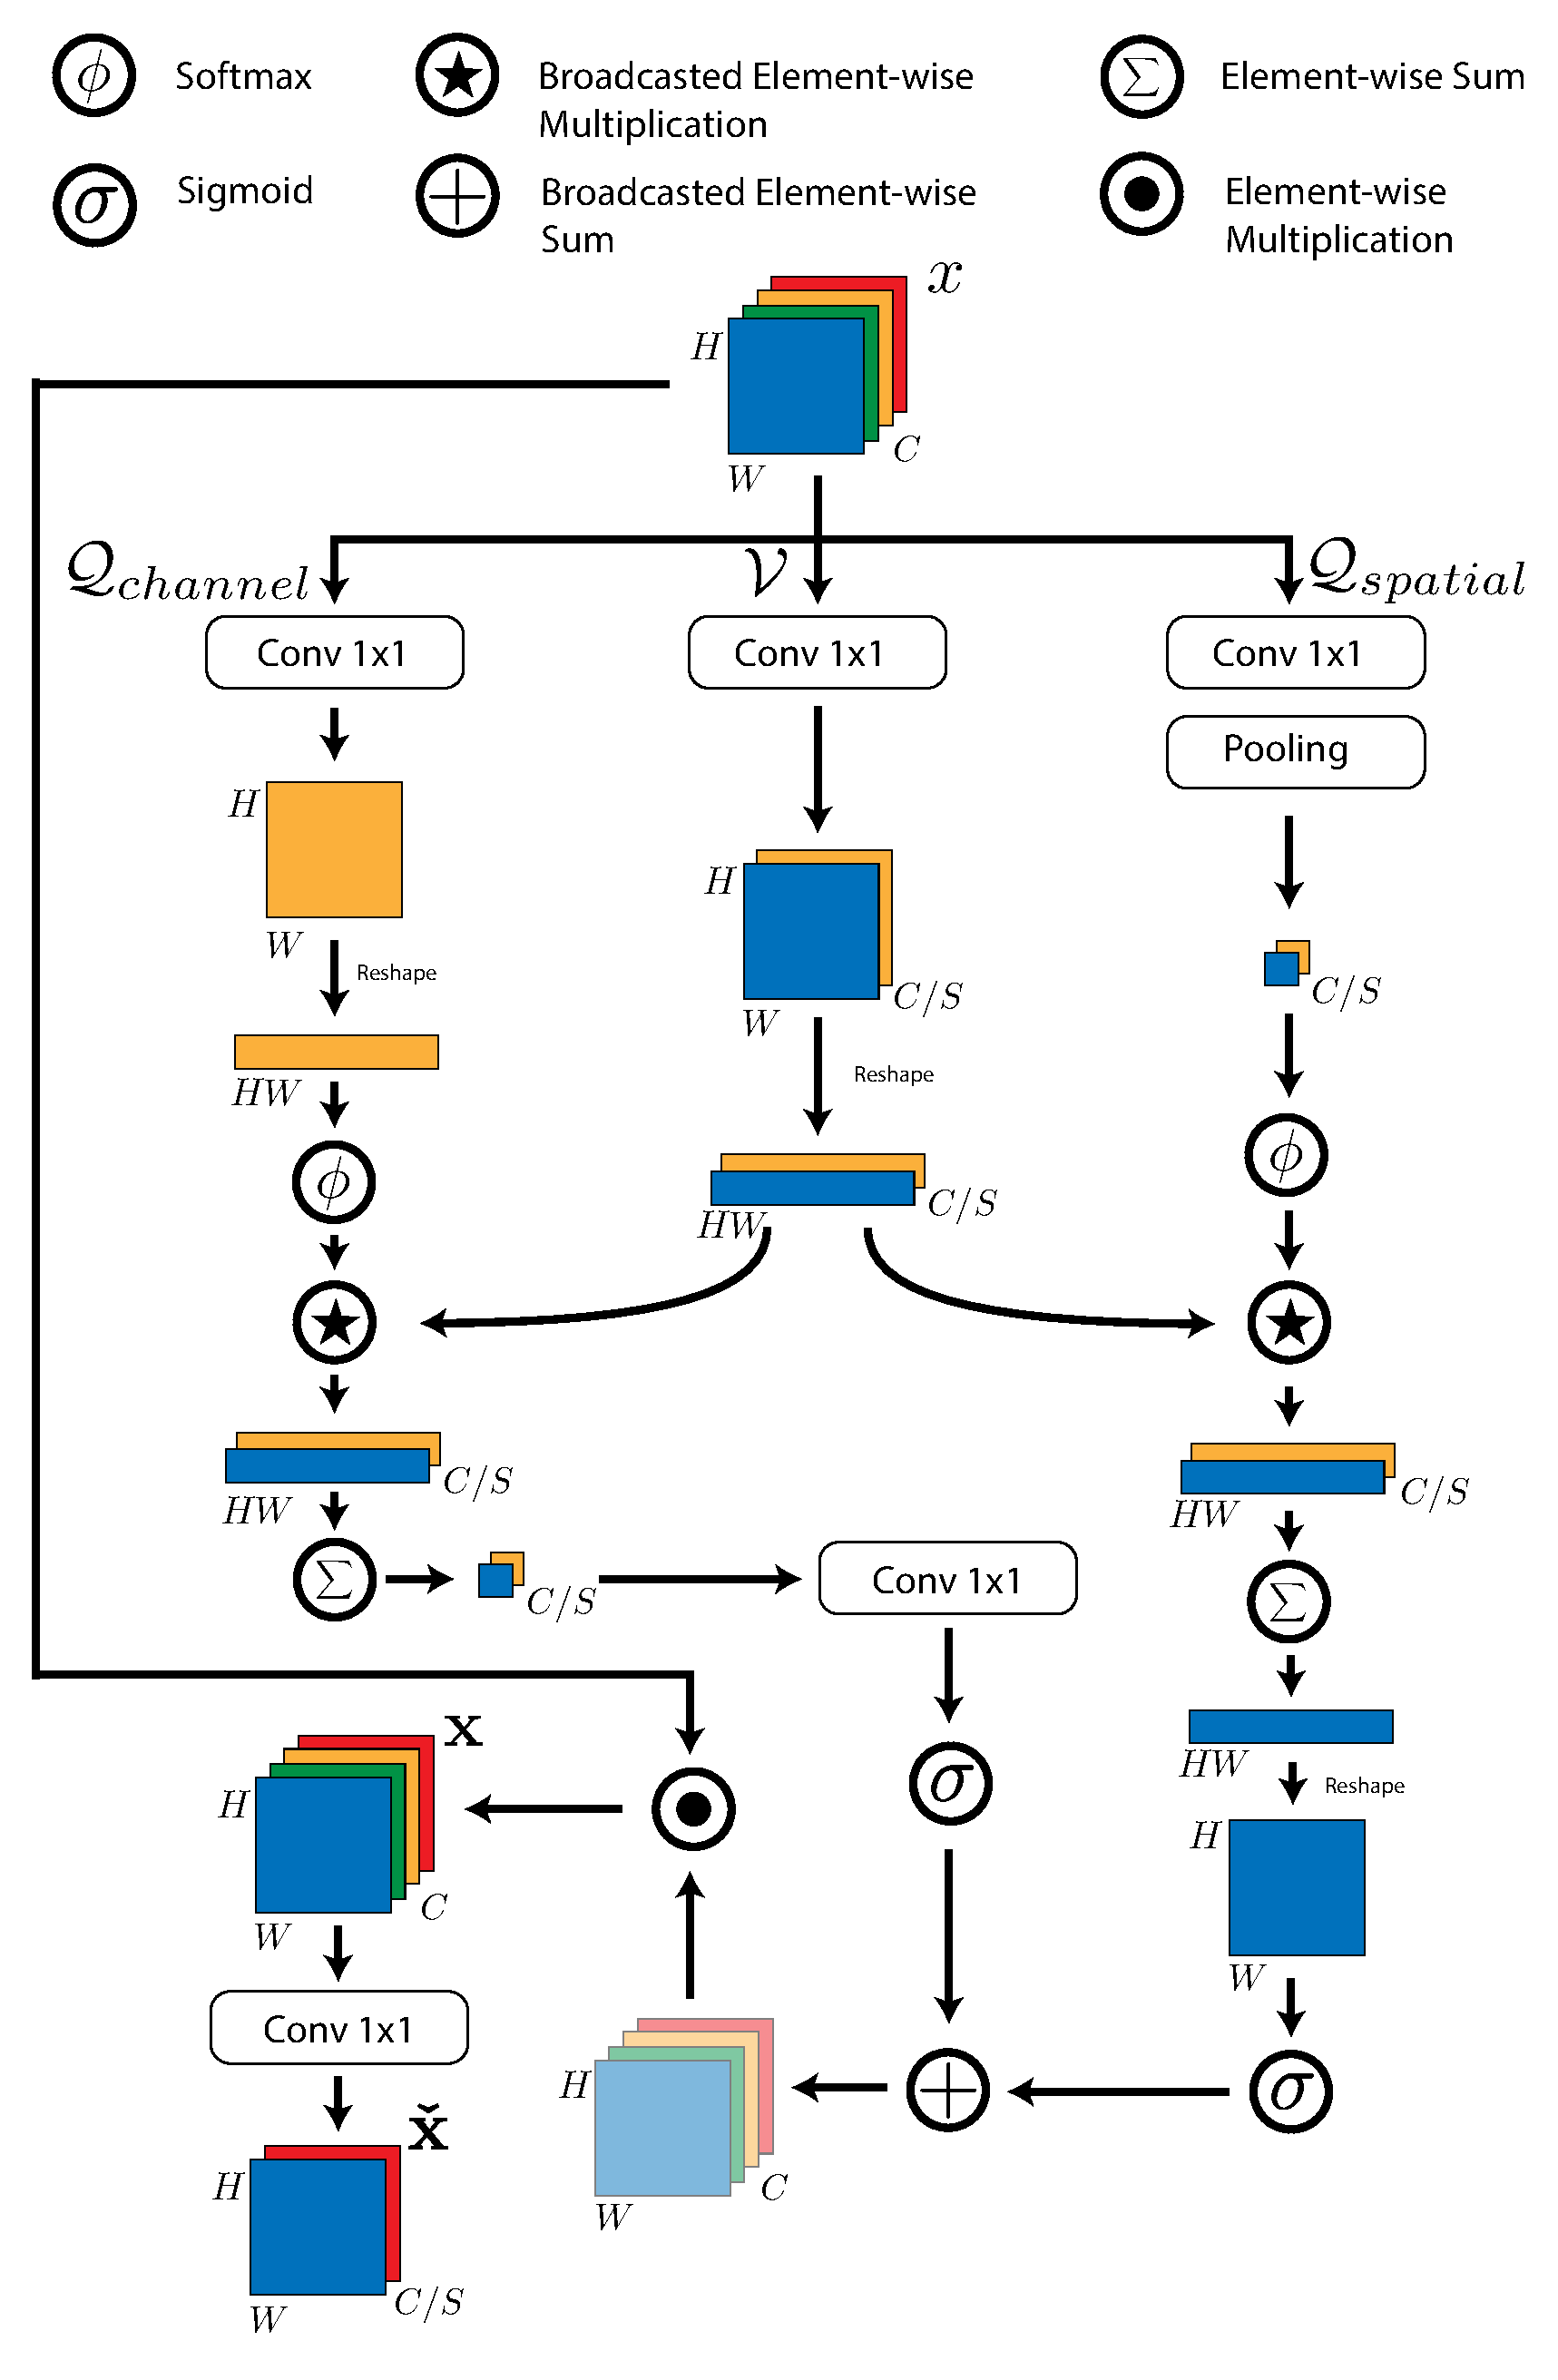
\includegraphics[width=0.9\textwidth]{figures/figure7.pdf}
   \caption{\textbf{Fast Mixed Filtration.} This block serves as a lightweight and effective attention mechanism. The input $x$ is filtered to produce the compressed representations $\boldsymbol{\check{x}}$. The broadcast and element-wise operations make this block efficient on CPU. }
   \label{fig:attention2}
\end{figure}
The dual-template features and the dual-search-region features used by the correlation module $CC(\cdot,\cdot)$ could each be the naive concatenation of the respective backbone features in each pair. However, we can potentially improve their combination by processing them with an efficient learnable layer that filters out less useful components while enhancing those important for the task at hand. This should hopefully lead to improved performance. In \ref{fig:all_ablation}(top), we have shown just that. Especially when tracking in the OOD case, naive feature concatenation severely underperforms the filtered combination.

We consider filtration mechanisms such as self-attention~\cite{vaswani2017attention}, only tailored to convolutional models since they tend to be more efficient on CPU. Polarized Self-Attention (PSA)~\cite{liu2021polarized} stands out as it functions as a filter and is a more powerful variant than CBAM~\cite{woo2018cbam}, with time complexity of $O(CWH)$, where $C$, $W$, $H$, are channel, width, and height of the tensor respectively. Another notable option is the CNN-ViT-based attention block MobileViTv3~\cite{wadekar2022mobilevitv3}, based on separable attention~\cite{mehta2022separable}. As shown in \ref{tab:att_comp}, we observed limited performance gain of MobileViTv3 over PSA, with relatively high FLOPs, parameters, and latency. We also noticed that PSA performs several matrix multiplications causing the latency on CPU to still be considerably high. This motivated the development of our \emph{Fast Mixed Filtration (FMF)}, a new and more efficient mixed filtration method. It is defined as follows
\begin{equation}\small
  \centering
  \label{eq:fast_pol_attention}
      \begin{aligned}   
          A_{ch}(x) &= \sigma(W_{ch}(\sum^{HW} W^V(x) \star \phi(W^Q_{ch}(x))  )) \; , \\ %channel-attention          
          A_{sp}(x) &= \sigma(\sum^{C} \phi(W^Q_{sp}(x)) \star W^V(x))\; ,\\ %spatial-attention
          \boldsymbol{x} &= (A_{ch} \oplus  A_{sp}) \odot x \; , \\
\end{aligned}
\end{equation}
where the notation means the following: $\sigma :=$ sigmoid, $\phi :=$ softmax, $W := \mathrm{conv}1 \times 1$,  $\star :=$ broadcasted element-wise multiplication, $\oplus :=$ broadcasted element-wise sum, $\odot :=$ element-wise multiplication, $\sum :=$ element-wise sum, $A_{ch} :=$ channel filter, $A_{sp} :=$ spatial filter, $V:=$ values, $Q:=$ queries, $x :=$ input  and $\boldsymbol{x} :=$ output. \ref{fig:attention2} depicts the schematic computation of the FMF layer.

Differently than PSA, the improved efficiency of FMF stems from reducing the computation overhead in \ref{eq:fast_pol_attention} by limiting the matrix operations to be broadcasted element-wise multiplications and element-wise summations across the vectors, and by setting $W^V_{sp}=W^V_{ch}=W^V$ for both $A_{ch}$ and $A_{sp}$, which further reduces the number of parameters. Similar to CBAM and PSA, we utilize a squeeze-and-excite framework~\cite{iandola2016squeezenet} to excite the relevant features within this block. As shown in \ref{tab:att_comp}, the latency of FMF is 0.4ms on a CPU, which has decreased from the 0.8ms of PSA, while not experiencing any performance loss.

We provide more details regarding the operations performed this block. Please refer to \ref{fig:attention2} for a schematic representation of FMT. When fusing the pair of feature maps coming either from the dual-template or the dual-search-region, we first concatenate the two feature maps resulting in a representation with $C+C=2C$ channels dimension. Here, we aim to enhance the most relevant features through this filtration process. We further want to compress the feature space from $2C \times H \times W \rightarrow C \times H \times W$; therefore, we choose a squeeze rate of $S = 2$. Here, $W^V$ and $W^Q_{sp}$ perform the squeeze for $V$ and $Q_{sp}$, respectively, for the channel and spatial filters, where an average pooling operation is applied to $W^Q_{sp}$ to decrease the spatial dimensions of $W^Q_{sp}$ from $C \times H \times W \rightarrow C \times 1 \times 1$.  Moreover, $W^Q_{ch}$ decreases the channel dimensions of $Q_{ch}$ from $2C \times H \times W \rightarrow 1 \times H \times W$. A softmax function, $\phi$, is applied to $W^Q_{ch}$ and $W^Q_{sp}$ to produce the channel and spatial filter masks, respectively. Also, broadcast element-wise multiplications, $\star$, and element-wise summation, $\sum$, are then performed between $W^V$ and $\phi(W^Q_{ch})$ and between $\phi (W^Q_{sp})$ and $W^V$ to produce channel and spatial filters of size $C \times 1 \times 1$ and $1 \times H \times W$, respectively. Since there was a squeeze operation on the channel filter, $W_{ch}$ is applied to the channel filter to unsqueeze the channel dimensions from $C \times 1 \times 1 \rightarrow 2C \times 1 \times 1$, followed by a Layer Normalization layer to normalize the feature distributions. Furthermore, a sigmoid operation, $\sigma$, is performed on these filters, and then a broadcast element-wise summation, $\oplus$, is performed to form a total filter map of size $2C \times H \times W$. An element-wise multiplication operation is performed between the full filter map and $x$ to enhance the most important features from $x$ to form the final output $\bold{x}$. After this mixed-filtration of $x$, we further readjust the number of channels from  $2C \times H \times W \rightarrow C \times H \times W$, giving us $\bold{\check{x} }$, to perform future correlations.

We use FMF with a squeeze rate $S=2$ (see \ref{fig:attention2}). In this way, if $x$ is the concatenated representation of the dual-template (i.e., $x_T \doteq F_D \cup F_T$) or of the dual-search-region (i.e., $x_t \doteq F_t \cup F_S$), then $\boldsymbol{x}$ is the filtered representation with channel dimension $2C$, to which we apply a channel dimension reduction from $2C$ to $C$, giving us $\boldsymbol{\check{x}}$ (i.e., $\boldsymbol{\check{x}}_T$ or $\boldsymbol{\check{x}}_t$).



\subsubsection{Pixel-wise Cross-Correlation.}
We combine the filtered dual representations $\boldsymbol{\check{x}}_T$ and $\boldsymbol{\check{x}}_t$ with the block $CC(\cdot)$, which is a pixel-wise cross-correlation. The output is then concatenated with $F_t$ and fed to a one-layer convolution to reduce the number of channels processed by the heads block.

\subsection{Heads Block}
Similar to~\cite{zhang2020ocean, borsuk2022fear}, tracking output is given by a classification head $CH(\cdot)$, and a bounding box regression head $BH(\cdot)$.
We use 2 lightweight convolution layers for $CH(\cdot)$ and 4 for $BH(\cdot)$.
The last layer of $CH(\cdot)$ has only 1 channel and predicts the foreground/background confidence score for the object, whereas the last layer of $BH(\cdot)$ has 4 channels, each responsible for predicting separate values ($x_{min}$, $y_{min}$, $x_{max}$, and $y_{max}$ for the object bounding box in the frame at time $t$), which is why we choose a higher number of convolution blocks for $BH(\cdot)$. Following~\cite{borsuk2022fear}, we keep the spatial resolution of these maps to 16 $\times$ 16. 

\begin{table}
\caption{Comparison of FLOPs, number of parameters, and latency when using MobileViTv3\cite{wadekar2022mobilevitv3}, Polarized Self-Attention\cite{liu2021polarized} and Fast Mixed Filtration, with their performances on AVisT \cite{noman2022avist} and LaSOT \cite{fan2021lasot}.}
  \label{tab:att_comp}
  \centering
  \scalebox{.65}{
  \begin{tabular}{c|c |c |c c c |c c | c c}
  \hline
  \multirow{2}{*}{Attention} & \multirow{2}{*}{FLOPs (G.)($\downarrow$)} & \multirow{2}{*}{Params (M.)($\downarrow$)} & \multicolumn{3}{c|}{Latency (ms)($\downarrow$)} & \multicolumn{2}{c|}{AVisT}   & \multicolumn{2}{c}{LaSOT} \\
  & & & CPU & GPU & Nano & AUC($\uparrow$) & OP50($\uparrow$) & AUC($\uparrow$)& Prec.($\uparrow$)\\
  \hline
  MobileViTv3 \cite{wadekar2022mobilevitv3} & 0.220 & 0.862 & 2.7 & 1.3 & 6.5 & 0.435 & 0.490 & 0.568 & 0.588 \\
  PSA \cite{liu2021polarized} & 0.051 & 0.526 & 0.8 & 0.25 & 4.3  & 0.457 & 0.529  & 0.567 & 0.588 \\
  \rowcolor{lightgray!20}FMF (ours) & 0.034 & 0.395 & 0.4 & 0.2 & 3.5 & 0.458 & 0.529 & 0.572 & 0.592 \\
  \hline
  \end{tabular}
  }
\end{table}

\section{Training Losses}

\subsection{Transitive Relation Loss (TRL)}
We help focussing the filtered representations of the dual-template and the dual-search-region on providing relational information that will aid the downstream tasks. To this end, we recognize that $\Omega(F_D,F_T)$ and $\Omega(F_t,F_S)$ should be ``similar'', since all the inputs contain information about the object. We introduce a loss  $\mathcal{L}_{TR}$ to encourage that. At the same time, given the high built in similarity between $F_D$ and $F_S$ (since $I_D \subset I_S$), to avoid learning representations that ignore the static template ($F_T$) and search region ($F_t$) information, we also add a regularization loss $\mathcal{L}_{Reg}$ that pulls the representations close to $F_t$. $\mathcal{L}_{Reg}$ is applied between $\Omega(F_D,F_T)$ and $F_t$.
$\mathcal{L}_{TR}$ and $\mathcal{L}_{Reg}$ are defined as
\begin{equation}\small
  \centering
  \label{eq:relation}
      \begin{aligned} 
          \mathcal{L}_{TR}&=\mathcal{D}(\Omega(F_D,F_T),\Omega(F_t,F_S)) \; , \\
          \mathcal{L}_{Reg}&=\mathcal{D}(\Omega(F_D,F_T),F_t)\; , \\
          \mathcal{D}(x_1, x_2)&=\dfrac{1}{2} (D(h_1(x_1), h_2(x_2)) +  D(h_1(x_2), h_2(x_1))), \\
          D(z_1,z_2)&=1 - \dfrac{z_1}{{||z_1||}_2} \cdot \dfrac{z_2}{{||z_2||}_2} \; ,
      \end{aligned}
\end{equation}
where $||\cdot||_2$ is the $\ell_2$-norm,  $h_1$ and $h_2$ are MLP projection heads used only during training, and $D(\cdot, \cdot)$ calculates the cosine distance. Moreover, $\mathcal{D}(\cdot,\cdot)$ is computed as in~\cite{chen2021exploring}, where we implement the stop-gradient operation to avoid degenerated solutions. We refer to the pair $\mathcal{L}_{TR}$ and $\mathcal{L}_{Reg}$ as the \emph{transitive relation loss (TRL)} since it is meant to bridge the similarities between template and search region images with the aid of the dynamic components so that the relevant relational differences can be highlighted by the downstream blocks for task purposes. The TRL loss improves tracking performance, especially when both components are used. See \ref{fig:all_ablation}(middle). Notably, in the OOD case, the AVisT \cite{noman2022avist} AUC improves from 43.7\% to 45.8\%.


\subsection{Total Tracking Loss} 
We use standard losses for the regression and classification heads. We use the $IoU$ loss~\cite{rezatofighi2019generalized}, $\mathcal{L}_{IoU}$, for the bounding box regression, $BH(\cdot)$, and the focal loss~\cite{lin2017focal}, $\mathcal{L}_{FL}$, for the classification head, $CH(\cdot)$. We refer to \cite{rezatofighi2019generalized,lin2017focal} for their definition.
The offline training of the tracker is therefore based on the \emph{total tracking loss}
\begin{equation} \small
  \centering
  \label{eq:overall_loss}
      % \begin{aligned}
      %     \mathcal{L} =  \lambda_{IoU} \mathcal{L}_{IoU} + \lambda_{FL} \mathcal{L}_{FL} + \lambda_{TR} \mathcal{L}_{TR} + \lambda_{Reg} \mathcal{L}_{Reg},
      % \end{aligned}
          \mathcal{L} =  \mathcal{L}_{IoU} + \lambda_{FL} \mathcal{L}_{FL} + \lambda_{TR} \mathcal{L}_{TR} + \lambda_{Reg} \mathcal{L}_{Reg},
\end{equation}
where we set $\lambda_{FL}$, $\lambda_{TR}$, and $\lambda_{Reg}$ to 1, 1/3, and 1/3, respectively.

\section{Dynamic Update} \label{sec:methods_update} 
Different strategies can be implemented for when to update the dynamic image template and dynamic search region image. \ref{tab:component_ablation_updates} reports our case-study focussing on parameter-free strategies, which suggests that different strategies are specific to their approaches and are not generally applicable. A simple yet effective strategy that gave us reliable performance is based on maintaining a running average of the classification scores $\overline{\rho }_t$
\begin{equation}
  \label{eq:sample_update}
          \overline{\rho }_t = (1-{\lambda}_{D}) \overline{\rho}_{t-1} +  {\lambda}_{D} {\rho}_t \; ,
\end{equation}
where, ${\rho}_t$ is the score at time $t$, and ${\lambda}_{D}$ is a momentum parameter, which we set to 0.25. We also start a counter, $C$, that when it reaches, let us say $N=60$ frames ($\approx$ 2 seconds), we compare the current classification score with the running average, and if ${\rho}_t > \overline{\rho }_{t-1}$, then we update the dynamic image components and reset the counter, otherwise we repeat the test at the next iteration. This strategy is effective, parameterless, and uses limited computational resources. \ref{alg:dynamic_update} describes the details of our dynamic sample update strategy with $N=60$ and ${\lambda}_{D} = 0.25$. This strategy is parameter-less and lightweight.

\begin{algorithm}
  \centering
  \caption{Dynamic Sample Update}\label{alg:dynamic_update}
  \begin{algorithmic}
    \State $t \gets 0$
    \State $x_t \gets $ sequence frame at time $t$
    \State $I_T \gets x_t$, $I_S \gets x_t$, $I_D \gets x_t$
    \State $init\_tracker(I_T)$ \Comment{initialize the tracker}
    \State $set\_dyn(I_S, I_D)$ \Comment{set the dynmaic samples}
    \State $C \gets 0$ \Comment{counter}
    \State $\overline{\rho}_t \gets 1$ \Comment{initialize average classification score}
  
    \While{$x_{t+1}$ is available}
      \State $C \gets C+1$ \Comment{increase the counter}
      \State $I_t \gets x_{t+1}$ \Comment{search-region} 
      \State ${\beta}_t, {\rho}_t \gets tracker(I_t)$ \Comment{ $\beta \gets$ bounding box}
      % \State \Comment{$\beta \gets$ bounding box}
      \State \Comment{$\rho \gets$ classification score}
      \If{$C \geq N$ \& ${\rho}_t > \overline{\rho }_{t}$}  \\ \Comment{$N \gets$ hyperparameter}
            \State $I_S, I_D \gets update(x_{t+1}, {\beta}_t)$ %
            \State $reset\_dyn(I_S, I_D)$ \\ \Comment{reset the dynmaic samples}
            \State $C \gets 0$
      \EndIf 
      \State $\overline{\rho }_t = (1-{\lambda}_{D}) \overline{\rho}_{t} +  {\lambda}_{D} {\rho}_t$ \\ \Comment{${\lambda}_{D} \gets$ hyperparameter}
      \EndWhile
  \end{algorithmic}
\end{algorithm}


\section{Dynamic Test-Time Adaptation} \label{sec:methods_tta}

To increase tracking performance, especially at OOD test-time, we introduce a dynamic test-time adaptation procedure based on a batch normalization (BN) correction tailored specifically to tracking. We applied this strategy to the classification and bounding box regression heads. First, BN layers are generally computed by the following equations:


\begin{equation}\small
    \centering
    \label{eq:bn}
        \begin{aligned}  
        BN(x) = \gamma \frac{x - E(x)}{\sqrt{Var(x)}} +  \beta ,
        \end{aligned}
\end{equation}
  
\begin{equation}\small
    \centering
    \label{eq:bn_running}
        \begin{aligned}  
            \overline{\mu}_t = (1-\alpha)  \overline{\mu}_{t-1} +  \alpha  {\mu}_t ,\\
            \overline{\sigma}_{t}^2 = (1-\alpha) \overline{\sigma}_{t-1}^2 +  \alpha {\sigma}_{t}^2 ,
        \end{aligned}
\end{equation}
    
where $x$ is the input feature, $E(x)$ and $Var(x)$ are the expected value and variance of $x$. $\gamma$ and $\beta$ are learnable parameters for scaling and shifting. The BN layers keep track of the running mean and variance through \ref{eq:bn_running}, where ${\mu}_t$ and ${\sigma}_{t}$ are current expected value and variance respectively, and $\overline{\mu}_t$ and $\overline{\sigma}_{t}$ are used for $E(x)$ and $Var(x)$, respectively. $\alpha$ is the momentum parameter. 
Estimating learnable parameters $\gamma$ and $\beta$ during testing would require a backward pass, with great detriment to the speed. Therefore, we propose a method that dynamically updates the BN statistics $E(x)$ and $Var(x)$ during testing, which has negligible computational overhead for maintaining speed.

Prior works have explored BN adaptation for classification purposes, with some using a backward pass for adaptation \cite{niu2022efficient, wang2020tent}, while others introduced backward-free adaptation \cite{pan2018two, schneider2020improving, mirza2022norm, li2016revisiting}. However, none are directly applicable for tracking. As we show in \ref{tab:tta_res}, applying a new Instance-Norm (IN) layer \cite{pan2018two} is expensive, and slows down the speed twofold without noticeable improvement. Additionally, the batch size for tracking remains 1, which is too small to make any significant improvement with \cite{schneider2020improving} that applies weighted momentum based on the target batch-size. Given the scale of our architecture and limited number of parameters, by replacing batch statistics with instance statistics, AdaBN \cite{li2016revisiting} does not improve the performance either. DUA \cite{mirza2022norm} uses source statistics as a prior for the incoming task but does not stay anchored to the source statistics, resulting in target statistics drifting away from the original distribution, causing performance drop. Therefore, we propose that BN statistics should be updated with weighted instance statistics while remaining anchored to the source statistics. This results in the following strategy
\begin{equation}
  \centering
  \label{eq:bn_update}
      \begin{aligned}  
          \overline{\mu}_{I,t} &= (1-\lambda{_{BN}}) \overline{\mu} +  \lambda{_{BN}} \mu_{I,t} \; ,\\
          \overline{\sigma}_{I,t}^2 &= (1-\lambda{_{BN}}) \overline{\sigma}^2 +  \lambda{_{BN}} \sigma_{I,t}^2 \; ,
      \end{aligned}
\end{equation}
where $\overline{\mu}$ and $\overline{\sigma}^2$ are the final running mean and variance of the model trained on the source data, respectively, and $\mu_{I,t}$, and $\sigma_{I,t}^2$ are mean and variance calculated from the instance at time $t$, respectively. $\overline{\mu}_{I,t}$ and $\overline{\sigma}_{I,t}^2$ are updated based on the current instance and used for feature normalization at time $t$. $ \lambda{_{BN}}$ is set to 0.1. This backward-free \emph{dynamic test-time adaptation (DTTA)} strategy is efficient with negligible difference in latency as shown in \ref{tab:tta_res}.



%%% Local Variables:
%%% mode: latex
%%% TeX-master: "../main"
%%% End:




